\documentclass[aspectratio=169]{beamer}
\usetheme{Madrid}
\usecolortheme{default}

\usepackage[T2A]{fontenc}
\usepackage[utf8]{inputenc}
\usepackage[russian,english]{babel}
\usepackage{graphicx}
\usepackage{booktabs}
\usepackage{array}
\usepackage{animate}
\usepackage{tikz}
\usetikzlibrary{arrows.meta,positioning}

\newcommand{\pipelinebox}[3]{%
  \node[draw=#1!80!black, fill=#1!10, rounded corners=2pt, align=center,
        minimum width=#2, minimum height=0.82cm, font=\scriptsize] (#3)
}
\newcommand{\optbox}[2]{%
  \node[draw=orange!85!black, fill=orange!12, rounded corners=2pt, align=center,
        minimum width=#1, minimum height=0.96cm, font=\scriptsize] (#2)
}

\title{Промежуточный отчёт по PushWorld}
\subtitle{Оптимизационный анализ пайплайна обучения}
\author{Иванкин Евгений, Сулиман Адам}
\date{}

\begin{document}

\begin{frame}
  \titlepage
\end{frame}

\begin{frame}{Что такое PushWorld}
  \centering
  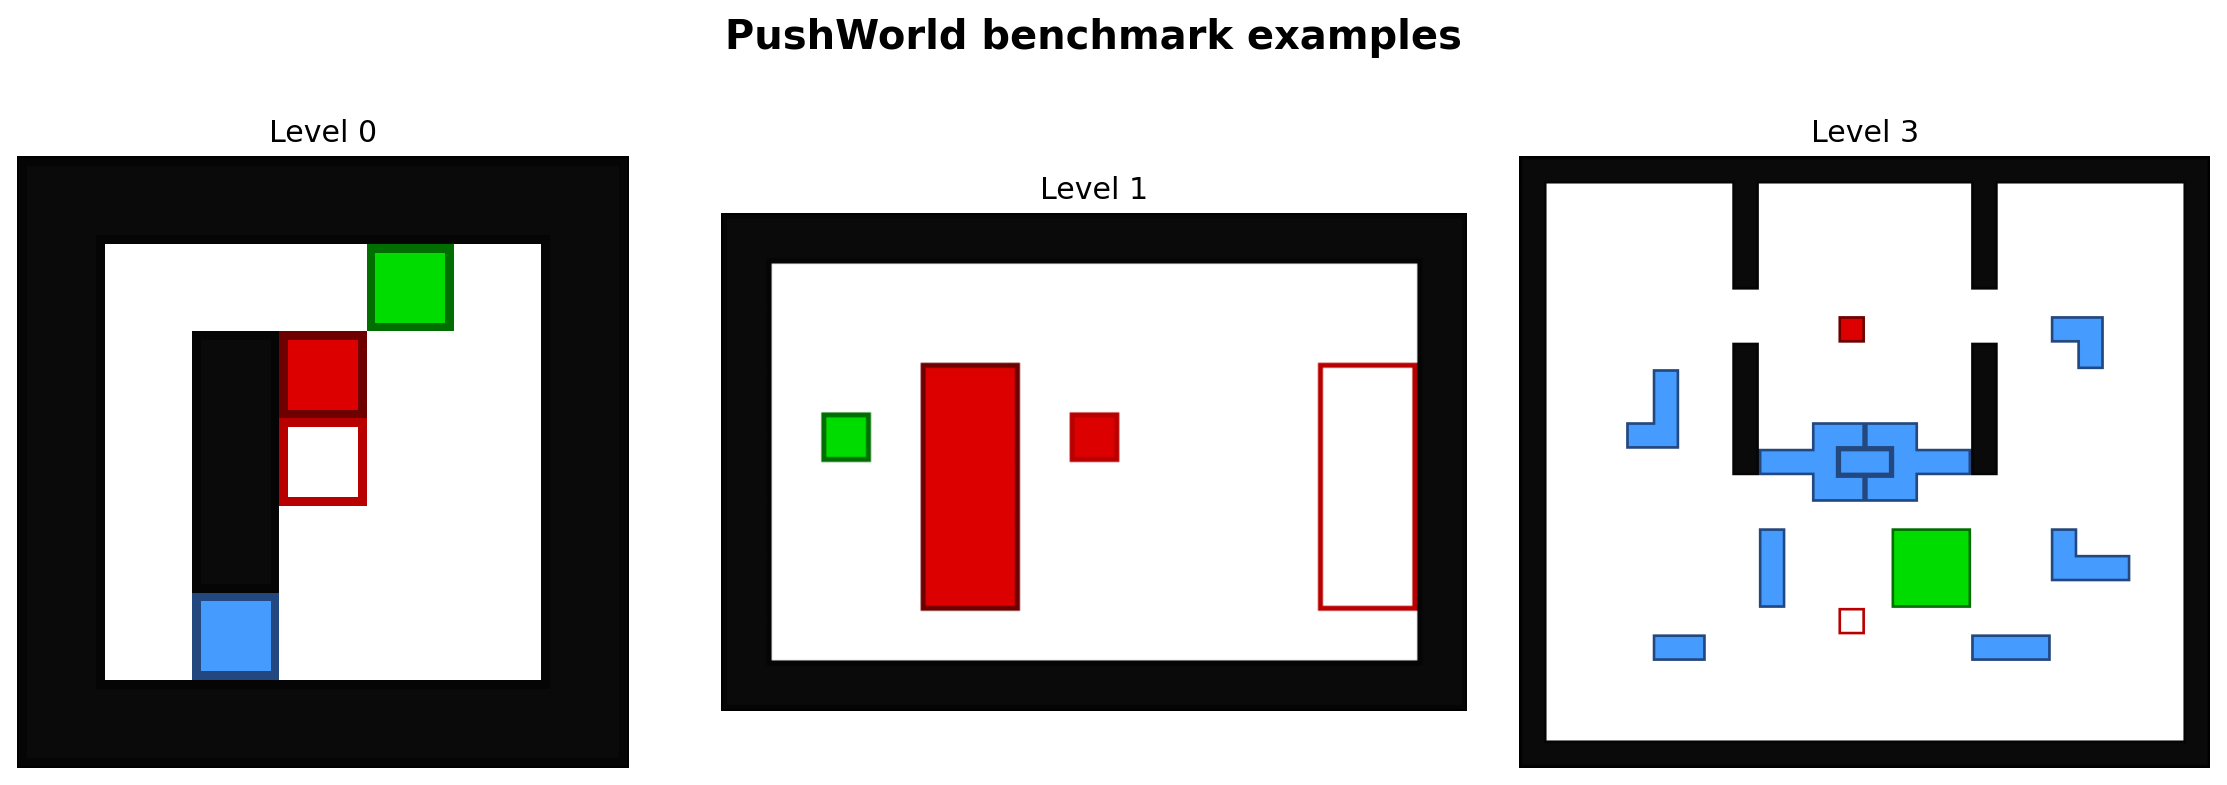
\includegraphics[height=0.54\textheight]{../assets/benchmark_overview.png}

  \vspace{0.6em}
  \begin{itemize}
    \item PushWorld --- planning benchmark: агент двигается по сетке и толкает объекты в целевые позиции.
    \item На сложных уровнях появляются инструменты, узкие проходы и длинные причинно-следственные цепочки.
    \item Для нас это удобный тест на то, где RL-пайплайн ломается по времени и по качеству.
  \end{itemize}
\end{frame}

\begin{frame}{Как выглядит решение в среде}
  \begin{columns}[T]
    \column{0.50\textwidth}
    \centering
    \animategraphics[autoplay,loop,width=0.84\linewidth]{3}{../assets/rollout_success/frame_}{000}{002}

    \column{0.50\textwidth}
    \centering
    \animategraphics[autoplay,loop,width=0.84\linewidth]{6}{../assets/rollout_fail/frame_}{000}{040}
  \end{columns}
\end{frame}

\begin{frame}{Бейзлайны слабые и медленные}
  \begin{itemize}
    \item PPO на RGB оказался нестабильным даже на 5 простых головоломках.
    \item DQN на том же наборе вел себя устойчивее, но работал очень медленно.
    \item Это были короткие прогоны порядка 100--200k итераций: по качеству это ещё не финальный вердикт, но слабость бейзлайнов уже видна.
    \item Для этого checkpoint важнее именно системный сигнал: куда уходит время и какой FPS даёт каждая конфигурация.
  \end{itemize}

  \vspace{0.9em}
  \centering
  \normalsize
  \begin{tabular}{@{}p{0.60\linewidth}cc@{}}
    \toprule
    Конфигурация & FPS & Успех \\
    \midrule
    PPO, RGB, 5 головоломок & 195 & 15\% \\
    DQN, RGB, 5 головоломок & 8 & 40\% \\
    \bottomrule
  \end{tabular}
\end{frame}

\begin{frame}{Что видит агент: RGB против planes}
  \centering
  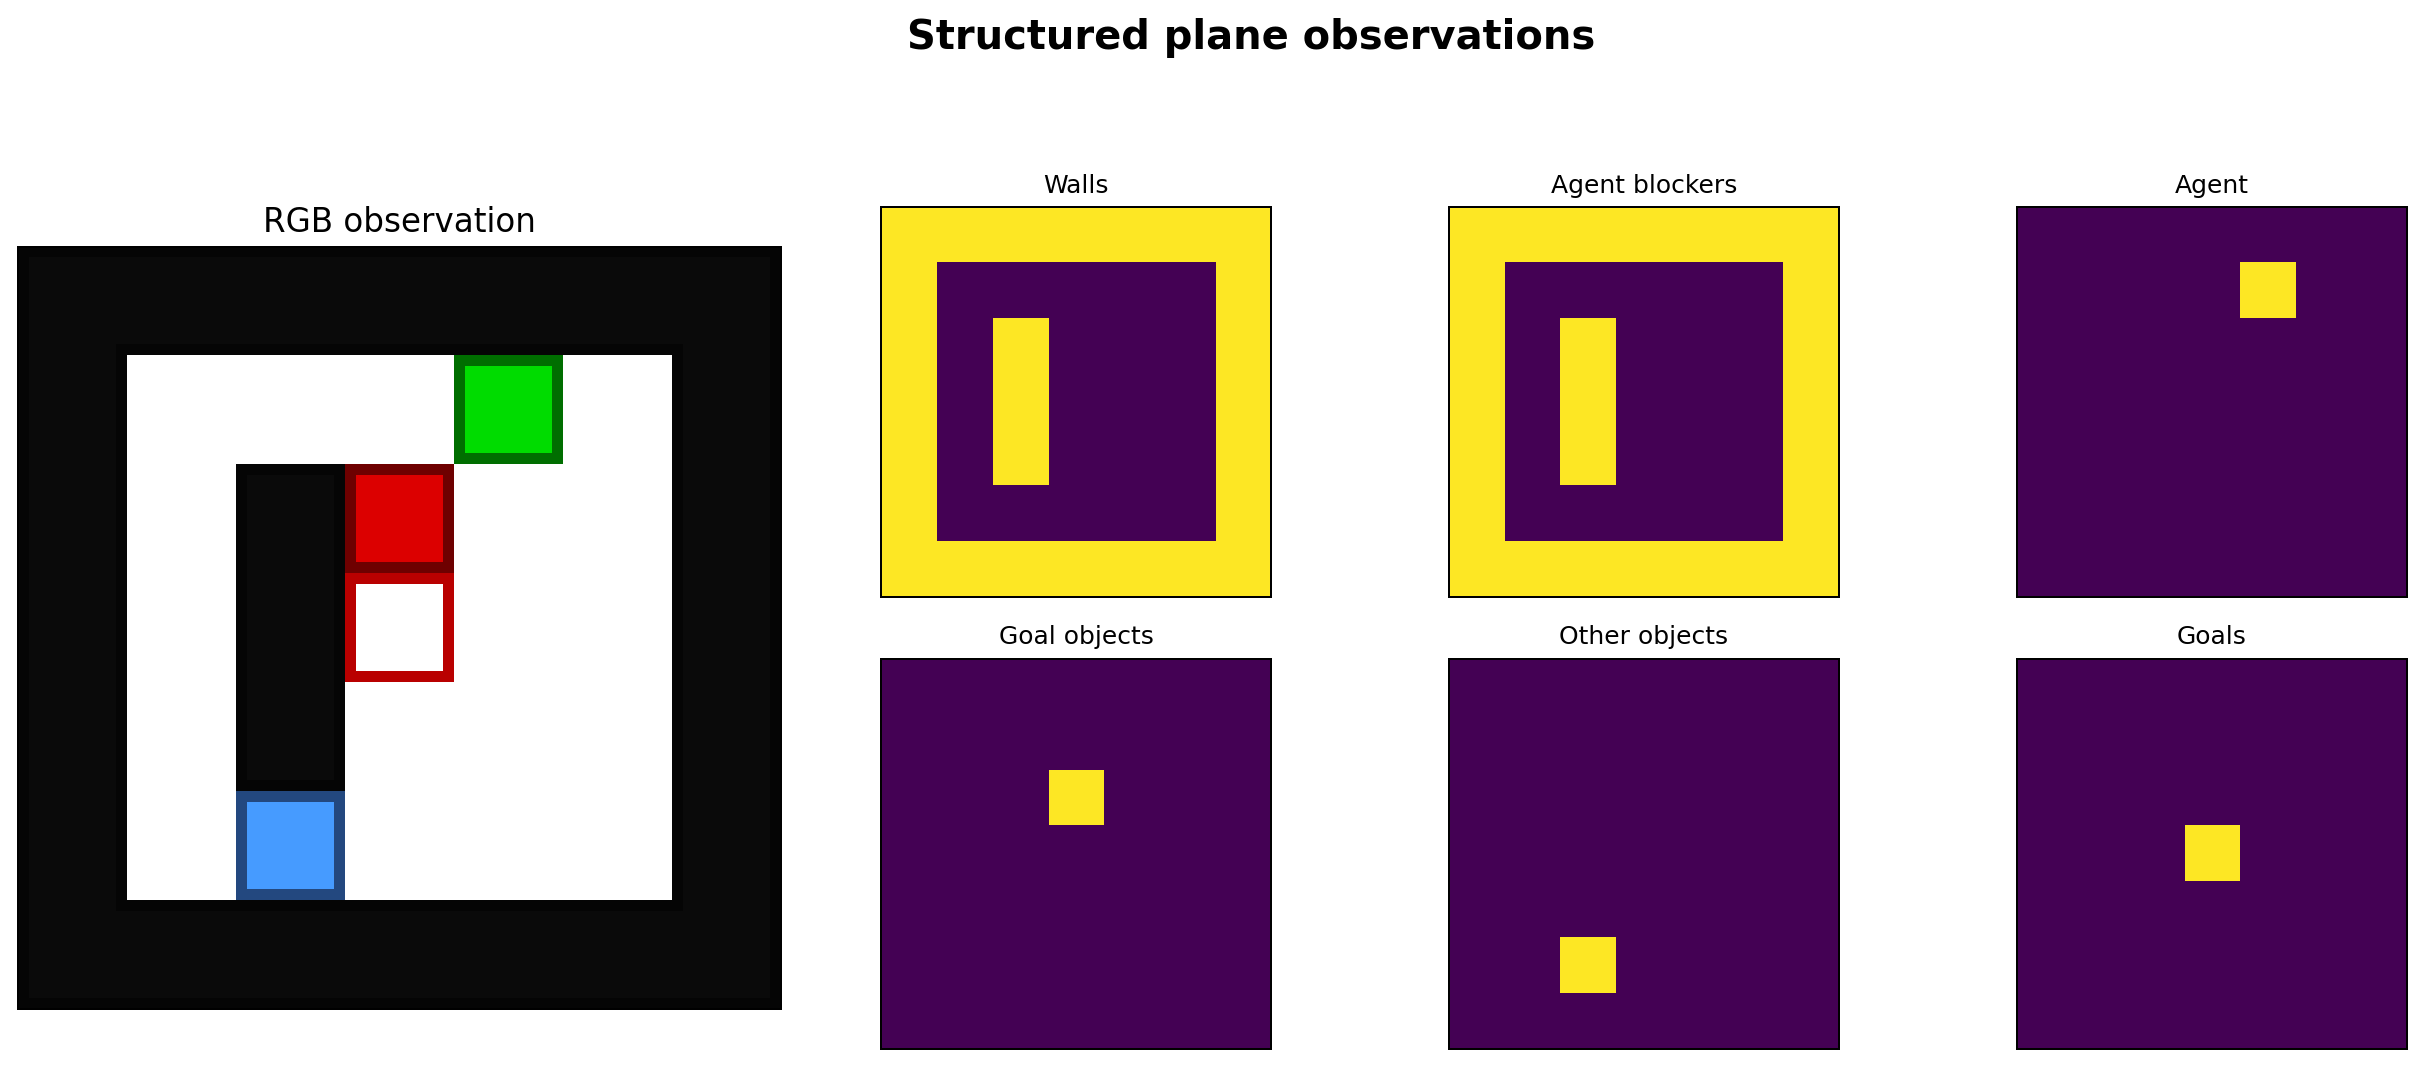
\includegraphics[height=0.55\textheight]{../assets/observation_modes.png}

  \vspace{0.3em}
  \small
  \begin{itemize}
    \item RGB требует рендерить большую картинку и гонять большие тензоры через replay/CNN.
    \item Plane-наблюдения оставляют только полезную структуру состояния.
    \item Ключевые числа: размер состояния 58{,}800 B \(\rightarrow\) 1{,}176 B; PPO 195 \(\rightarrow\) 586 FPS; DQN 8 \(\rightarrow\) 161.7 FPS.
  \end{itemize}
\end{frame}

\begin{frame}{После planes среда уже не главный bottleneck}
  \centering
  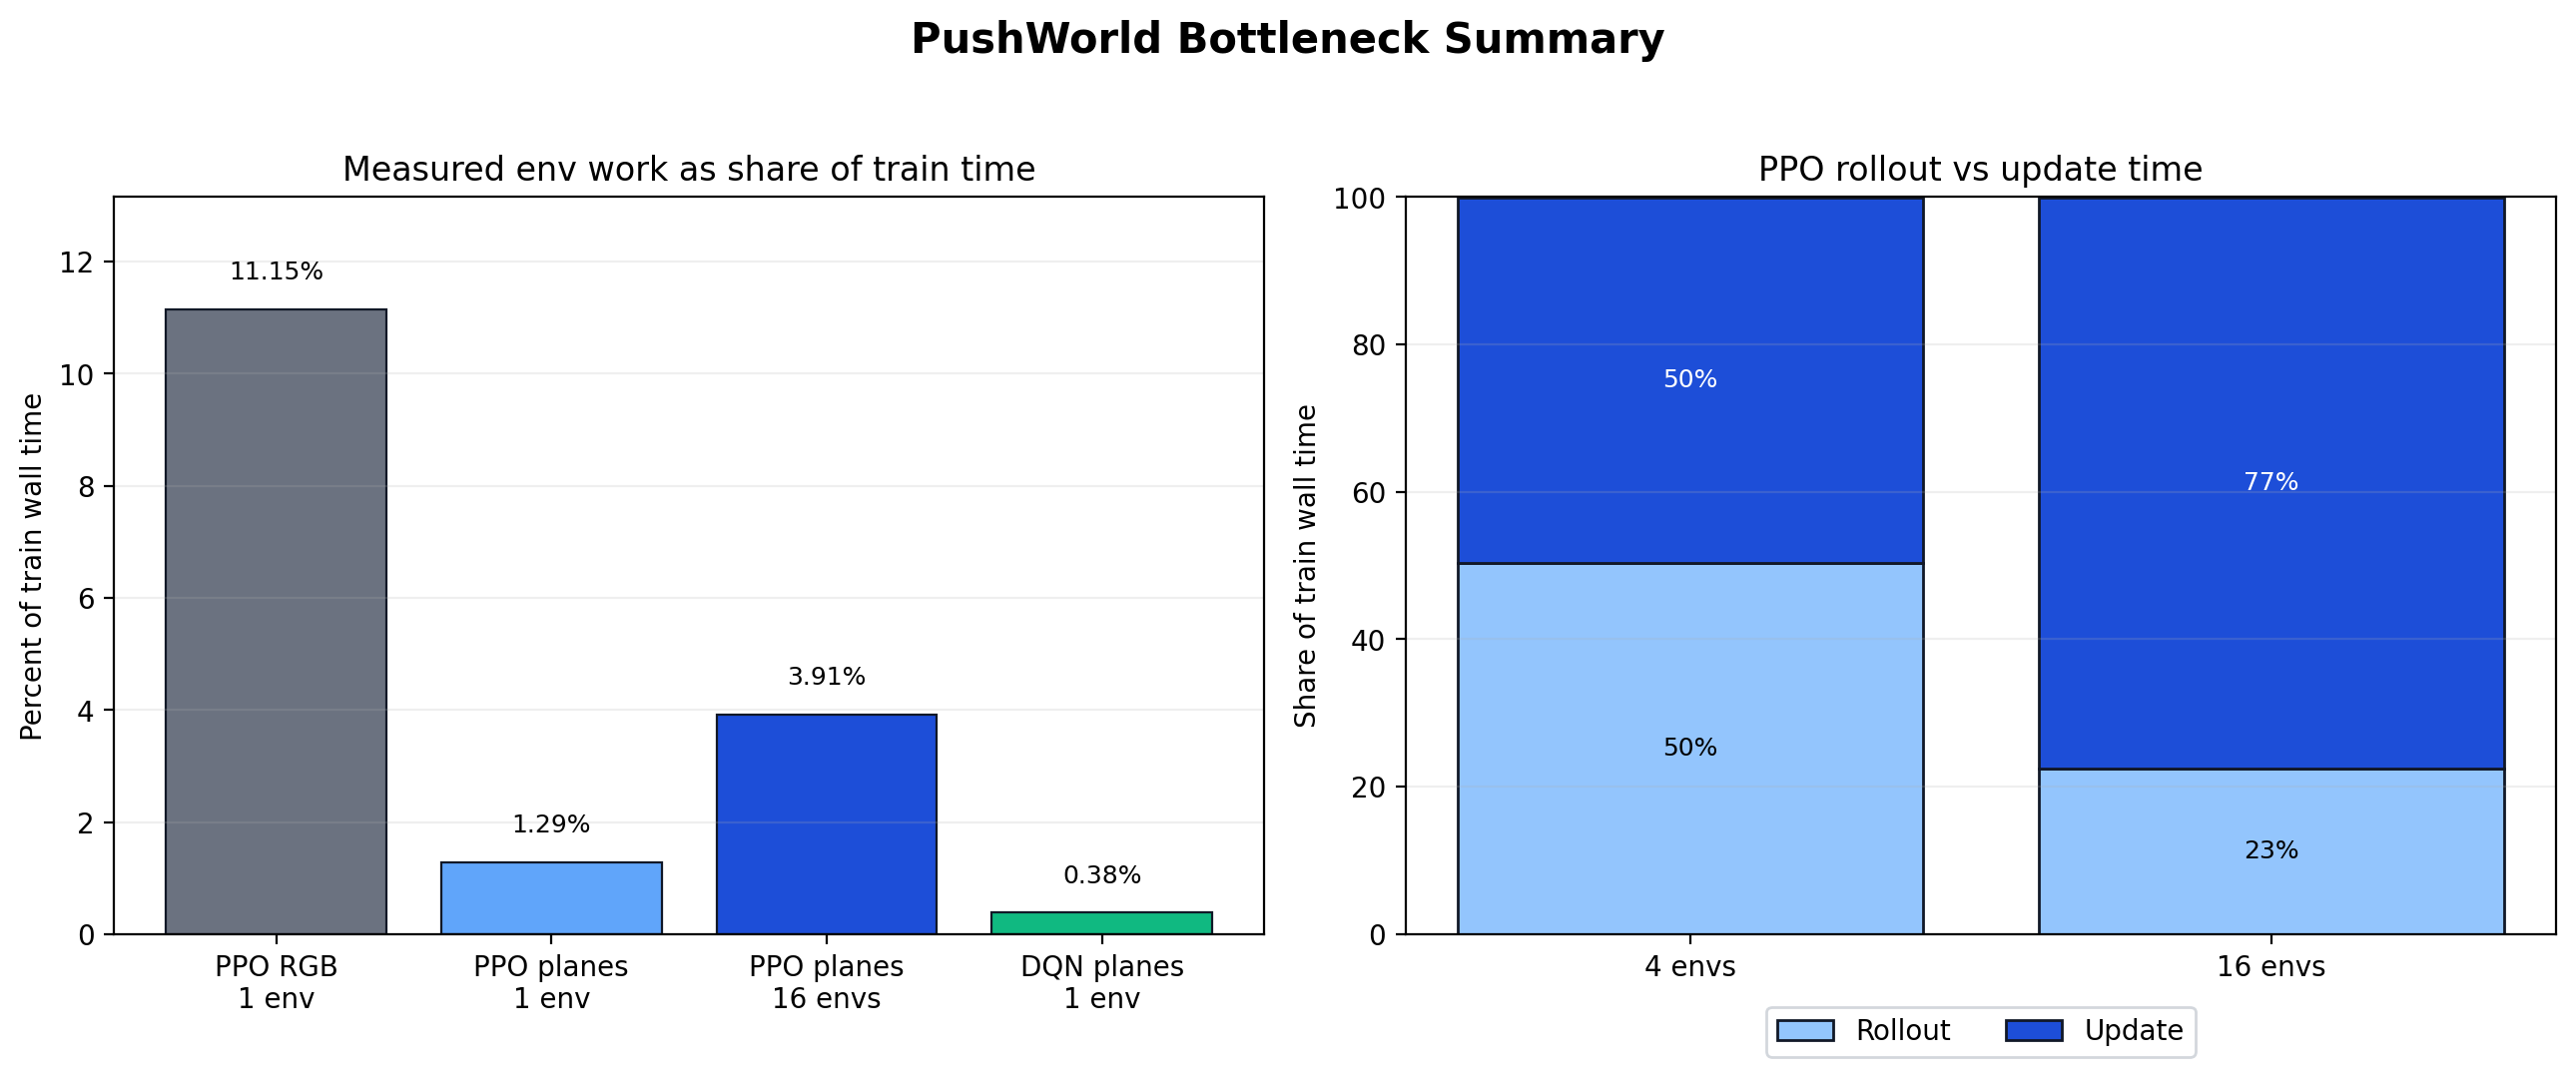
\includegraphics[height=0.50\textheight]{../assets/bottleneck_summary.png}

  \vspace{0.4em}
  \begin{itemize}
    \item PPO, RGB: среда занимает \textbf{11.15\%} train time. PPO, planes: только \textbf{1.29\%}.
    \item PPO, planes + 16 envs: \textbf{77.4\%} времени уже уходит в update. DQN, planes: среда занимает всего \textbf{0.38\%}, update --- \textbf{76.0\%}.
    \item Итог: сейчас главный bottleneck --- не симуляция среды, а learner/update stack. Поэтому переписывать среду на GPU прямо сейчас преждевременно.
  \end{itemize}
\end{frame}

\begin{frame}{Ещё одна оптимизация: \texttt{torch.compile}}
  \begin{columns}[T]
    \column{0.54\textwidth}
    \begin{itemize}
      \item Мы проверили уже не только representation-level оптимизации, но и model-side оптимизацию.
      \item \texttt{torch.compile} заметно ускоряет чистый forward pass.
      \item Но end-to-end training step ускоряется совсем слабо.
      \item Значит, оставшийся bottleneck шире, чем просто скорость инференса.
    \end{itemize}

    \column{0.46\textwidth}
    \centering
    \begin{tabular}{@{}lccc@{}}
      \toprule
      Batch & Метрика & Eager & Compile \\
      \midrule
      256 & Infer/s & 1055.6 & 1643.6 \\
      256 & Train/s & 345.7 & 359.1 \\
      512 & Infer/s & 614.5 & 878.7 \\
      512 & Train/s & 201.6 & 208.3 \\
      \bottomrule
    \end{tabular}

    \vspace{0.5em}
    \small
    Ускорение inference: \textbf{1.43x--1.56x}\\
    Ускорение training: только \textbf{1.03x--1.04x}
  \end{columns}
\end{frame}

\begin{frame}{Пайплайн, который мы ускоряем}
  \small
  \begin{center}
  \begin{tikzpicture}[>=Latex]
    \node[draw=blue!80!black, fill=blue!10, rounded corners=2pt, align=center, minimum width=2.0cm, minimum height=0.9cm, font=\scriptsize] (state) at (0,0) {PushWorld\\state};
    \node[draw=blue!80!black, fill=blue!10, rounded corners=2pt, align=center, minimum width=2.0cm, minimum height=0.9cm, font=\scriptsize] (obs) at (2.75,0) {Plane\\observation};
    \node[draw=blue!80!black, fill=blue!10, rounded corners=2pt, align=center, minimum width=2.0cm, minimum height=0.9cm, font=\scriptsize] (policy) at (5.5,0) {Policy\\model};
    \node[draw=blue!80!black, fill=blue!10, rounded corners=2pt, align=center, minimum width=2.0cm, minimum height=0.9cm, font=\scriptsize] (rollout) at (8.25,0) {Rollout /\\replay};
    \node[draw=blue!80!black, fill=blue!10, rounded corners=2pt, align=center, minimum width=2.0cm, minimum height=0.9cm, font=\scriptsize] (update) at (11.0,0) {Learner\\update};

    \draw[->, thick] (state) -- (obs);
    \draw[->, thick] (obs) -- (policy);
    \draw[->, thick] (policy) -- (rollout);
    \draw[->, thick] (rollout) -- (update);
  \end{tikzpicture}
  \end{center}

  \begin{columns}[T]
    \column{0.48\textwidth}
    \textbf{Уже ускорили}
    \begin{itemize}
      \item RGB rendering \(\rightarrow\) compact planes.
      \item Observation payload: 58{,}800 B \(\rightarrow\) 1{,}176 B.
      \item PPO: 195 \(\rightarrow\) 586 FPS; DQN: 8 \(\rightarrow\) 161.7 FPS.
    \end{itemize}

    \column{0.52\textwidth}
    \textbf{Следующие шаги для этого pipeline}
    \begin{itemize}
      \item Goal-conditioned planes + relabeling \href{https://arxiv.org/abs/1707.01495}{[HER]}.
      \item Update profiling: dataloader, policy forward/backward, optimizer step.
      \item AMP, rollout length, minibatch size, update epochs, replay/buffer layout.
      \item Метрика: success/time и update seconds per \(10^5\) env steps.
    \end{itemize}
  \end{columns}
\end{frame}

\begin{frame}{Transformer policy pipeline}
  \small
  \begin{center}
  \begin{tikzpicture}[>=Latex]
    \node[draw=green!60!black, fill=green!10, rounded corners=2pt, align=center, minimum width=2.0cm, minimum height=0.9cm, font=\scriptsize] (planner) at (0,0) {planner\\solutions};
    \node[draw=green!60!black, fill=green!10, rounded corners=2pt, align=center, minimum width=2.2cm, minimum height=0.9cm, font=\scriptsize] (data) at (2.8,0) {state-action\\dataset};
    \node[draw=green!60!black, fill=green!10, rounded corners=2pt, align=center, minimum width=2.2cm, minimum height=0.9cm, font=\scriptsize] (enc) at (5.6,0) {plane encoder\\+ transformer};
    \node[draw=green!60!black, fill=green!10, rounded corners=2pt, align=center, minimum width=2.2cm, minimum height=0.9cm, font=\scriptsize] (heads) at (8.4,0) {action +\\distance heads};
    \node[draw=green!60!black, fill=green!10, rounded corners=2pt, align=center, minimum width=2.2cm, minimum height=0.9cm, font=\scriptsize] (search) at (11.2,0) {greedy /\\beam search};
    \draw[->, thick] (planner) -- (data);
    \draw[->, thick] (data) -- (enc);
    \draw[->, thick] (enc) -- (heads);
    \draw[->, thick] (heads) -- (search);
  \end{tikzpicture}
  \end{center}

  \begin{itemize}
    \item Цель: ускорять не environment stepping, а supervised training и autoregressive search around policy.
    \item Метрики: action accuracy, greedy solve rate, beam solve rate, states/sec during search, GPU utilization.
    \item Основа: Sokoban transformer-policy + GPU rollout direction \href{https://timallanwheeler.com/blog/category/sokoban/}{[Wheeler]}.
  \end{itemize}
\end{frame}

\begin{frame}{Transformer policy: конкретный план оптимизации}
  \small
  \begin{enumerate}
    \item Dataset first: экспортировать planner traces и кэшировать plane tensors, чтобы training не ждал парсер/симулятор.
    \item Model ablation: CNN-only no-history baseline \(\rightarrow\) transformer over last \(k\) states \(\rightarrow\) distance head.
    \item Training optimization: фиксированный dataloader, AMP, \texttt{torch.compile}, larger batches; мерить samples/sec и validation.
    \item Search optimization: сначала greedy, затем beam width 8/16/32; батчировать scoring всех beam candidates одним forward.
    \item Cache policy inputs: не пересчитывать encoder для одинаковых states; хранить visited states и logits/distance.
    \item Остановиться, если beam search time растёт быстрее solve rate; тогда оптимизировать ranking head, а не width.
  \end{enumerate}
\end{frame}

\begin{frame}{Hybrid solver pipeline}
  \small
  \begin{center}
  \begin{tikzpicture}[>=Latex]
    \node[draw=cyan!60!black, fill=cyan!10, rounded corners=2pt, align=center, minimum width=2.0cm, minimum height=0.9cm, font=\scriptsize] (state) at (0,0) {current\\state};
    \node[draw=cyan!60!black, fill=cyan!10, rounded corners=2pt, align=center, minimum width=2.1cm, minimum height=0.9cm, font=\scriptsize] (plan) at (2.7,0) {planner\\subgoals};
    \node[draw=cyan!60!black, fill=cyan!10, rounded corners=2pt, align=center, minimum width=2.2cm, minimum height=0.9cm, font=\scriptsize] (exec) at (5.5,0) {goal-conditioned\\executor};
    \node[draw=cyan!60!black, fill=cyan!10, rounded corners=2pt, align=center, minimum width=2.2cm, minimum height=0.9cm, font=\scriptsize] (monitor) at (8.3,0) {monitor\\progress};
    \node[draw=cyan!60!black, fill=cyan!10, rounded corners=2pt, align=center, minimum width=2.2cm, minimum height=0.9cm, font=\scriptsize] (replan) at (11.1,0) {accept or\\replan};
    \draw[->, thick] (state) -- (plan);
    \draw[->, thick] (plan) -- (exec);
    \draw[->, thick] (exec) -- (monitor);
    \draw[->, thick] (monitor) -- (replan);
    \draw[->, thick] (replan.north) -- ++(0,0.75) -| node[pos=0.26, above, font=\scriptsize] {new subgoal} (plan.north);
  \end{tikzpicture}
  \end{center}

  \begin{itemize}
    \item Цель: заменить дорогой full search на planner skeleton + fast learned local execution.
    \item Метрики: subgoal success, replans per puzzle, planner time vs executor time, solved puzzles per minute.
    \item Близкая идея декомпозиции: planner задаёт структуру, learned follower исполняет локальные шаги \href{https://arxiv.org/abs/2310.01207}{[Learn to Follow]}.
  \end{itemize}
\end{frame}

\begin{frame}{Hybrid solver: конкретный план оптимизации}
  \small
  \begin{enumerate}
    \item Offline subgoals: взять solution traces и нарезать на достижимые partial goals через каждые \(k\) действий.
    \item Executor baseline: goal-conditioned CNN policy учится по imitation / relabeling на Level 0 subgoals.
    \item Interface profiling: отдельно мерить planner call time, executor inference time, env stepping, replanning overhead.
    \item Reduce planner calls: cache subgoal plans, replan only after timeout or distance-to-subgoal regression.
    \item Learn ranker/value: если planner даёт несколько candidates, ранжировать их моделью вместо полного rollout search.
    \item Ablation: planner-only, executor-only, hybrid without ranker, hybrid with ranker.
  \end{enumerate}
\end{frame}

\begin{frame}{RAGEN pipeline: LLM-agent RL}
  \small
  \begin{center}
  \begin{tikzpicture}[>=Latex]
    \node[draw=violet!80!black, fill=violet!10, rounded corners=2pt, align=center, minimum width=2.0cm, minimum height=0.9cm, font=\scriptsize] (env) at (0,0) {PushWorld\\Gym wrapper};
    \node[draw=violet!80!black, fill=violet!10, rounded corners=2pt, align=center, minimum width=2.1cm, minimum height=0.9cm, font=\scriptsize] (prompt) at (2.7,0) {text state\\+ prompt};
    \node[draw=violet!80!black, fill=violet!10, rounded corners=2pt, align=center, minimum width=2.1cm, minimum height=0.9cm, font=\scriptsize] (llm) at (5.4,0) {LLM\\reason + action};
    \node[draw=violet!80!black, fill=violet!10, rounded corners=2pt, align=center, minimum width=2.1cm, minimum height=0.9cm, font=\scriptsize] (traj) at (8.1,0) {trajectory\\reward};
    \node[draw=violet!80!black, fill=violet!10, rounded corners=2pt, align=center, minimum width=2.1cm, minimum height=0.9cm, font=\scriptsize] (upd) at (10.8,0) {StarPO\\update};
    \draw[->, thick] (env) -- (prompt);
    \draw[->, thick] (prompt) -- (llm);
    \draw[->, thick] (llm) -- (traj);
    \draw[->, thick] (traj) -- (upd);
    \draw[->, thick] (upd.north) -- ++(0,0.75) -| node[pos=0.26, above, font=\scriptsize] {new policy} (llm.north);
  \end{tikzpicture}
  \end{center}

  \begin{itemize}
    \item RAGEN trains LLM agents through multi-turn environment interaction: state text \(\rightarrow\) reasoning/action \(\rightarrow\) reward \(\rightarrow\) policy update \href{https://arxiv.org/abs/2504.20073}{[RAGEN]}.
    \item PushWorld adaptation: Gym wrapper, deterministic text renderer, strict action parser, reward/success adapter.
    \item Baselines: fixed prompt without fine-tune on 256 episodes; then LoRA/StarPO on a small Level 0 split.
  \end{itemize}
\end{frame}

\begin{frame}{RAGEN pipeline: план оптимизации}
  \small
  \begin{enumerate}
    \item Baseline profiling: wall time, tokens/sec, tokens/episode, env-step time, generation time, update time, GPU memory.
    \item Prompt compression: verbose state vs compact ASCII planes; cap reasoning tokens; require one-token action answer.
    \item Rollout batching: batch \(P\) initial states \(\times N\) samples per state through vLLM; measure GPU utilization.
    \item Runtime settings: reproduce paper's vLLM no-enforce-eager / graph-retention setup, then tune Ray workers and env placement.
    \item Training cost: compare no-finetune, LoRA, full update by success/time and memory/time-to-first-improvement.
    \item Rollout filtering: keep high-variance/high-signal prompt groups; measure time-to-target success, not just final reward.
  \end{enumerate}

  \vspace{0.25em}
  \scriptsize
  RAGEN reports runtime/resource context, not a full throughput table: Figure 5 has Sokoban PPO total-time plots; Appendix C.2 gives H100/A100 + vLLM/Ray/FSDP settings; Appendix H compares LoRA resources \href{https://arxiv.org/pdf/2504.20073}{[paper]}.
\end{frame}

\begin{frame}{Источники и ориентиры}
  \small
  \begin{itemize}
    \item \textbf{[1]} M. Andrychowicz et al. \textit{Hindsight Experience Replay}. NeurIPS, 2017.
    
    \href{https://arxiv.org/abs/1707.01495}{arxiv.org/abs/1707.01495}

    \item \textbf{[2]} T. Wheeler. Серия материалов о Sokoban, sequence modeling и GPU rollout.
    
    \href{https://timallanwheeler.com/blog/category/sokoban/}{timallanwheeler.com/blog/category/sokoban/}

    \item \textbf{[3]} \textit{Learn to Follow: Decentralized Lifelong Multi-agent Pathfinding via Planning and Learning}, 2023.
    
    \href{https://arxiv.org/abs/2310.01207}{arxiv.org/abs/2310.01207}

    \item \textbf{[4]} Z. Wang et al. \textit{RAGEN: Understanding Self-Evolution in LLM Agents via Multi-Turn Reinforcement Learning}, 2025.

    \href{https://arxiv.org/abs/2504.20073}{arxiv.org/abs/2504.20073}
    \quad
    \href{https://github.com/mll-lab-nu/RAGEN}{github.com/mll-lab-nu/RAGEN}
  \end{itemize}

\end{frame}

\begin{frame}{Код и материалы}
  \centering
  
\includegraphics[height=0.58\textheight]{../assets/github_qr.png}

  \vspace{0.6em}
  \large
  \href{https://github.com/eivankin/pushworld}{github.com/eivankin/pushworld}
\end{frame}

\end{document}
